% Provenance (never printed): see sources/outline_sources.md (Year 3:
% moments of inertia and gravity fields; impact cratering and crater dating;
% volcanism and tectonics on Mars, Venus, Io and the icy moons).
% Brief: sources/book5/BRIEFS.md, ch. 26. Curves from figdata/bachelor-3/
% two_layer_planet.py (two-layer interiors of the Earth, Mars, the Moon and
% Mercury from mean density and moment of inertia) and crater_sfd.py
% (the Ivanov production function and the Hartmann-Neukum chronology of
% Mars from the Craterstats configuration, the lunar chronology of Neukum,
% Hartmann's equilibrium density, and two invented Martian plains whose
% counts are drawn once from a Poisson law). Exercise and problem values in
% the Book 5 scratch calculator calc/ch26.py. Plains A and B are invented.
\chapter{Intérieurs et surfaces planétaires}\label{ch:b3:planetary-interiors-surfaces}

Vue à la jumelle, la Lune présente deux sortes de terrains. Les hautes terres
claires sont couvertes de cratères, des cratères sur des cratères~: elles ont
été saturées de grands cratères lors d'un bombardement intense qui s'est achevé
il y a environ 3.8~Ga. Les maria sombres, des plaines remplies de lave entre 4.2 et
1.2~Ga, en portent beaucoup moins. Les missions Apollo et Luna ont
ramené des roches des deux, et leurs âges radiométriques ont transformé la
densité de cratères d'une surface en horloge. Cette horloge sert aujourd'hui
à dater des plaines sur Mars, Mercure et les lunes glacées, dont aucune roche
n'a encore été rapportée. Ce chapitre lit les intérieurs des planètes dans leur
champ de gravité, leur rotation et leurs marées, puis leurs surfaces dans leurs
cratères, leurs volcans et leurs failles.
% ledger: french:highlands, nasa:moon-core, marchi:neukum

\begin{recall}
Le facteur de moment d'inertie $C = I/MR^2$, le modèle à deux couches d'une
planète construit à partir de celui-ci et de la masse volumique moyenne, les
planètes telluriques et les planètes géantes sont dans le volume de première
année, dans son chapitre de planétologie comparée~; les panaches mantelliques et
les grandes provinces magmatiques, dans son chapitre sur les points chauds. La différenciation planétaire et les météorites sont dans le volume de deuxième
année, dans son chapitre sur la formation des planètes. Le \omterm{def:b3:gravity-geodesy:j2}{facteur de forme dynamique}
$J_2$, la \omterm{thm:b3:gravity-geodesy:maccullagh}{formule de MacCullagh} et la flexure de la lithosphère sont dans ce
volume, dans son chapitre sur la gravité et la géodésie~; le \omterm{def:b3:mantle-convection:rayleigh}{nombre de Rayleigh}, dans son
chapitre sur la convection mantellique. Les marées, les lois de Kepler et les modules
d'élasticité sont dans les volumes de physique~; la distribution de Poisson, dans les
volumes de mathématiques.
\end{recall}

\section{Intérieurs issus de la gravité, de la rotation et des marées}\label{sec:b3:planetary-interiors-surfaces:interiors}

La masse d'une planète, déduite de l'orbite d'une lune ou d'une sonde, donne sa
masse volumique moyenne~; la précession de son axe et son $J_2$ donnent son moment
d'inertie. La proposition à deux couches du volume de première année transforme
ces deux nombres en un noyau, mais seulement une fois une masse volumique du
manteau choisie~: deux mesures ne peuvent pas fixer trois inconnues.

\begin{omfigure}
\centering
\begin{tikzpicture}
\begin{axis}[width=0.78\linewidth, height=0.46\linewidth,
  xmin=3000, xmax=16000, ymin=0, ymax=1,
  xlabel={masse volumique du noyau $\rho_c$ (\unit{kg.m^{-3}})},
  ylabel={rayon du noyau / rayon de la planète $x$},
  tick label style={font=\scriptsize}, label style={font=\small},
  scaled x ticks=false, xtick={4000,6000,8000,10000,12000,14000,16000},
  xticklabels={4000,6000,8000,10\,000,12\,000,14\,000,16\,000}]
\addplot[thick, omDef] table[x=rho_c, y=x] {figdata/out/bachelor-3-two_layer_planet-curve-Earth.dat};
\addplot[thick, red!70!black] table[x=rho_c, y=x] {figdata/out/bachelor-3-two_layer_planet-curve-Mars.dat};
\addplot[thick, black!60, dashed] table[x=rho_c, y=x] {figdata/out/bachelor-3-two_layer_planet-curve-Moon.dat};
\addplot[thick, orange!80!black] table[x=rho_c, y=x] {figdata/out/bachelor-3-two_layer_planet-curve-Mercury.dat};
\addplot[only marks, mark=*, mark size=2pt, black] table[x=rho_c, y=x] {figdata/out/bachelor-3-two_layer_planet-points.dat};
\node[font=\scriptsize, omDef, anchor=south west] at (axis cs:12600,0.55) {Terre};
\node[font=\scriptsize, red!70!black, anchor=south west] at (axis cs:6600,0.55) {Mars};
\node[font=\scriptsize, black!70, anchor=south west] at (axis cs:11000,0.2) {Lune};
\node[font=\scriptsize, orange!80!black, anchor=south west] at (axis cs:7300,0.83) {Mercure};
\end{axis}
\end{tikzpicture}
\par\smallskip{\small Les modèles à deux couches permis par la masse volumique moyenne et
le facteur de moment d'inertie de quatre corps~: chaque courbe parcourt les
masses volumiques de manteau possibles, un manteau plus dense laissant un noyau
plus petit et plus dense. Les points marquent les rayons de noyau mesurés~: celui de la Terre par la sismologie,
celui de Mars par le sismomètre d'InSight, le noyau interne et la couche
liquide de la Lune, celui de Mercure par le champ de gravité
de la sonde MESSENGER.}\label{fig:b3:planetary-interiors-surfaces:two-layer}
\end{omfigure}
% ledger: planet:Earth.density, planet:Mars.density, planet:Moon.density, planet:Mercury.density, earth:MoI, nasa:mars, nasa:moon, nasa:mercury, data:prem, jpl:insight-interior, nasa:moon-core, agu:mercury-core

Chaque planète donne une courbe, non un point. Pour Mars, le rayon de noyau de
\qty{1830}{km} mesuré par InSight sélectionne un manteau de \qty{3460}{kg.m^{-3}}
et un noyau de \qty{6460}{kg.m^{-3}}. Pour Mercure, le noyau d'environ
\qty{2000}{km} de rayon occupe 82~\% du rayon. La courbe de la Lune est
presque plate~: son $C = 0.394$ est si proche de $\tfrac25$ qu'un petit noyau
de n'importe quelle densité convient, et une variation de $0.001$ de $C$ déplace le
rayon du noyau de plus d'un facteur deux (\cref{exo:b3:planetary-interiors-surfaces:10}).
La gravité seule ne voit pas un petit noyau~; les marées et les ondes sismiques le peuvent.
% ledger: jpl:insight-interior, agu:mercury-core, nasa:moon

\begin{definition}[Nombre de Love]\label{def:b3:planetary-interiors-surfaces:love-number}
Lorsqu'un potentiel de marée de degré~2 agit sur une planète, la planète se déforme et
sa masse redistribuée ajoute un potentiel qui lui est propre. Le \emph{nombre de
Love}\index{nombre de Love} $k_2$ est le rapport de ce potentiel ajouté au
potentiel de marée, tous deux pris à la surface de la planète.
\end{definition}

Une planète rigide a $k_2 = 0$~; une planète fluide de densité uniforme cède
entièrement, avec $k_2 = \tfrac32$. Entre les deux, le nombre mesure la part
de la planète qui cède.

\begin{proposition}[Nombre de Love d'une sphère élastique homogène]\label{prop:b3:planetary-interiors-surfaces:kelvin}
Une sphère incompressible de masse volumique uniforme $\rho$, de rayon $R$, de
gravité de surface $g$ et de rigidité $\mu$ a
\[
  k_2 = \frac{3/2}{1 + \dfrac{19\mu}{2\rho g R}} .
\]
\end{proposition}

Ce résultat, dû à Kelvin, est admis. Le rapport $\mu/\rho gR$ compare la rigidité
élastique à l'auto-gravitation qui ramène le renflement de marée~: les petites
planètes sont rigides, les grandes cèdent. Pour Mars, $\rho gR =
\qty{4.97e10}{Pa}$~; avec la rigidité du manteau supérieur terrestre,
\qty{67}{GPa} à \qty{80}{km} de profondeur dans le modèle de Terre de référence, la
formule donne $k_2 = 0.109$. Le suivi de la sonde en orbite Mars Global Surveyor
a mesuré la marée solaire de Mars~: $k_2 = 0.153 \pm 0.017$, trop
grand pour un noyau de fer solide. Au moins la partie externe du noyau est
liquide, et son rayon a été placé entre 1520 et \qty{1840}{km} en 2003.
% ledger: nasa:mars, const:G, data:prem, yoder:mars-k2

Les sismomètres ont tranché la question. La sonde InSight a enregistré
des séismes martiens et détecté des ondes réfléchies au sommet du noyau~: rayon
\qty{1830}{km}, sous un manteau profond de \qty{1560}{km} et une croûte épaisse de 20 à
\qty{37}{km}. Sur la Lune, les sismomètres installés par les astronautes d'Apollo
ont enregistré des séismes lunaires, les plus profonds, à plusieurs centaines de
kilomètres, étant déclenchés par les marées terrestres. Le noyau lunaire est
aujourd'hui décrit comme un noyau interne solide riche en fer, de \qty{240}{km} de rayon,
entouré d'une coque de fer liquide épaisse de \qty{90}{km}, elle-même surmontée
d'une couche partiellement fondue.
% ledger: jpl:insight-interior, nasa:moonquakes, nasa:moon-core

\section{Cratérisation par impact}\label{sec:b3:planetary-interiors-surfaces:impacts}

Un corps venu de l'espace frappe une planète à une vitesse au moins égale
à la vitesse de libération de celle-ci, soit \qty{11.2}{km.s^{-1}} pour la Terre~; les astéroïdes atteignent typiquement
la Terre à une vitesse de 15 à \qty{25}{km.s^{-1}}, et les comètes jusqu'à
\qty{60}{km.s^{-1}}. À \qty{20}{km.s^{-1}}, chaque kilogramme transporte
\qty{2e8}{J}, soit une cinquantaine de fois l'énergie d'un kilogramme d'explosif. L'impact
envoie une onde de choc dans le sol et dans le projectile, qui fond et se vaporise~;
derrière le choc, la roche est mise en mouvement vers l'extérieur, et un cratère
s'ouvre en quelques secondes.
% ledger: french:velocities, french:table21

\begin{definition}[Cratère transitoire, cratère simple, cratère complexe, couverture d'éjectas]\label{def:b3:planetary-interiors-surfaces:crater-morphology}
Le \emph{cratère transitoire}\index{cratère transitoire} est la cavité en forme de cuvette
ouverte par l'écoulement d'excavation au moment où elle cesse de grandir~; sa profondeur vaut environ
le tiers de son diamètre. Un \emph{cratère
simple}\index{cratère simple} est une cuvette à bord surélevé, le cratère transitoire étant à peine
modifié~: ses parois raides s'effondrent vers l'intérieur en une lentille de brèche. Un
\emph{cratère complexe}\index{cratère complexe} est un cratère plus grand dont la cuvette transitoire
s'est effondrée~: le plancher s'est soulevé en un pic central, le bord a glissé vers l'intérieur le long de
terrasses, et le plancher est plat. La \emph{couverture
d'éjectas}\index{couverture d'éjectas} est la nappe de roche excavée projetée
au-delà du bord et déposée autour du cratère.
\end{definition}
% ledger: french:transient, french:transition

\begin{omfigure}
\centering
\begin{tikzpicture}[x=0.55cm, y=0.55cm, font=\scriptsize, >=stealth]
\def\simpleprofile{(-6,0) -- (-3.6,0) .. controls (-3.0,0.45) .. (-2.6,0.55) .. controls (-1.8,-2.6) and (1.8,-2.6) .. (2.6,0.55) .. controls (3.0,0.45) .. (3.6,0) -- (6,0)}
\def\complexprofile{(-7,0) -- (-5.4,0) -- (-4.6,0.5) -- (-4.0,-0.3) -- (-3.6,-0.25) -- (-3.1,-1.0) -- (-2.7,-0.95) -- (-2.3,-1.5) -- (-0.8,-1.5) -- (-0.5,-0.6) -- (0,-0.3) -- (0.5,-0.6) -- (0.8,-1.5) -- (2.3,-1.5) -- (2.7,-0.95) -- (3.1,-1.0) -- (3.6,-0.25) -- (4.0,-0.3) -- (4.6,0.5) -- (5.4,0) -- (7,0)}
\begin{scope}
\fill[black!8] \simpleprofile -- (6,-4) -- (-6,-4) -- cycle;
\begin{scope}
\clip \simpleprofile -- (6,-4) -- (-6,-4) -- cycle;
\draw[black!45] (-6,-1.2) -- (6,-1.2) (-6,-2.4) -- (6,-2.4);
\fill[black!28] (-2.25,-0.5) .. controls (-1.2,-2.05) and (1.2,-2.05) .. (2.25,-0.5) .. controls (1.0,-0.8) and (-1.0,-0.8) .. (-2.25,-0.5);
\end{scope}
\fill[black!40] (-5.2,0) -- (-2.6,0.55) -- (-3.6,0.12) -- cycle;
\fill[black!40] (5.2,0) -- (2.6,0.55) -- (3.6,0.12) -- cycle;
\draw[thick] \simpleprofile;
\draw[omDef, dashed, thick] (-2.4,0.35) .. controls (-1.6,-3.1) and (1.6,-3.1) .. (2.4,0.35);
\node[anchor=south] at (0,1.2) {cratère simple};
\node[fill=black!28, inner sep=1pt] at (0,-1.45) {lentille de brèche};
\node[omDef, anchor=north, fill=black!8, inner sep=1pt] at (0,-2.65) {cratère transitoire};
\draw[->] (-4.9,1.2) node[anchor=south] {éjectas} -- (-4.3,0.2);
\draw[->] (3.6,1.4) node[anchor=south] {bord surélevé} -- (2.8,0.62);
\end{scope}
\begin{scope}[xshift=7.6cm]
\fill[black!8] \complexprofile -- (7,-4) -- (-7,-4) -- cycle;
\begin{scope}
\clip \complexprofile -- (7,-4) -- (-7,-4) -- cycle;
\draw[black!45] (-7,-1.2) -- (7,-1.2);
\draw[black!45] (-7,-2.4) -- (-1.3,-2.4) .. controls (-0.6,-2.4) and (-0.5,-1.75) .. (0,-1.75) .. controls (0.5,-1.75) and (0.6,-2.4) .. (1.3,-2.4) -- (7,-2.4);
\draw[black!45] (-7,-3.4) -- (-1.6,-3.4) .. controls (-0.7,-3.4) and (-0.6,-2.7) .. (0,-2.7) .. controls (0.6,-2.7) and (0.7,-3.4) .. (1.6,-3.4) -- (7,-3.4);
\draw[black!70] (-4.0,-0.3) -- (-3.2,-2.0) (4.0,-0.3) -- (3.2,-2.0) (-3.1,-1.0) -- (-2.5,-2.2) (3.1,-1.0) -- (2.5,-2.2);
\end{scope}
\draw[thick] \complexprofile;
\node[anchor=south] at (0,1.5) {cratère complexe};
\draw[->] (1.4,0.75) node[anchor=south west, inner sep=1pt] {pic central} -- (0.25,-0.2);
\node[anchor=north, fill=black!8, inner sep=0.5pt] at (-1.3,-1.6) {plancher plat};
\draw[->] (-3.2,1.4) node[anchor=south] {terrasses} -- (-3.8,-0.12);
\draw[->] (-5.6,-0.6) node[anchor=east, fill=black!8, inner sep=1pt, xshift=4pt] {failles} -- (-3.65,-1.35);
\node[anchor=north, fill=black!8, inner sep=1pt] at (0,-3.55) {couches soulevées};
\end{scope}
\end{tikzpicture}
\par\smallskip{\small Coupes transversales d'un \omterm{def:b3:planetary-interiors-surfaces:crater-morphology}{cratère simple} et d'un \omterm{def:b3:planetary-interiors-surfaces:crater-morphology}{cratère complexe}
dans une roche stratifiée (non à l'échelle). À gauche~: la cuvette d'un \omterm{def:b3:planetary-interiors-surfaces:crater-morphology}{cratère simple}
conserve la forme du \omterm{def:b3:planetary-interiors-surfaces:crater-morphology}{cratère transitoire} (en pointillés), partiellement comblée par une
lentille de brèche, sous un bord surélevé et une \omterm{def:b3:planetary-interiors-surfaces:crater-morphology}{couverture d'éjectas}. À droite~: dans un
\omterm{def:b3:planetary-interiors-surfaces:crater-morphology}{cratère complexe}, la cuvette transitoire s'est effondrée~; les couches profondes se sont
élevées sous un pic central, et le bord a glissé vers l'intérieur le long de failles
pour former des terrasses.}\label{fig:b3:planetary-interiors-surfaces:craters}
\end{omfigure}
% ledger: french:transient, french:transition

\begin{omfigure}
\centering
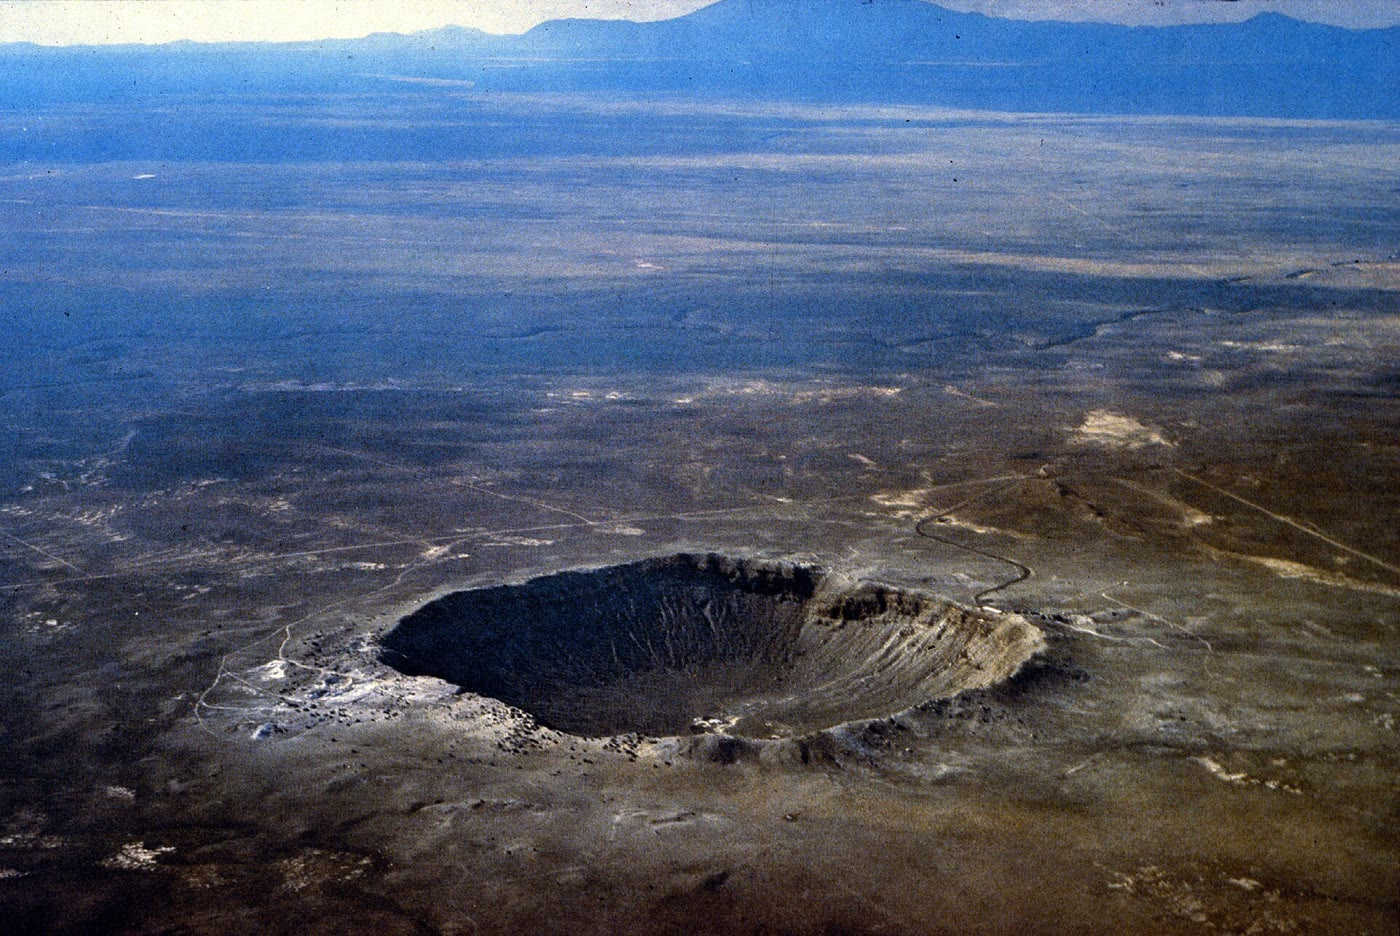
\includegraphics[width=0.66\linewidth]{images/book5/b3-barringer-crater.jpg}
\par\smallskip{\small Barringer Meteor Crater, Arizona, un \omterm{def:b3:planetary-interiors-surfaces:crater-morphology}{cratère simple}
de \qty{1.2}{km} de diamètre, formé il y a environ 50~000 ans par une
météorite de fer d'environ \qty{30}{m} de diamètre~; le bord domine le plateau
et la \omterm{def:b3:planetary-interiors-surfaces:crater-morphology}{couverture d'éjectas} s'étend autour de lui. Photographie aérienne,
USGS/D.~Roddy, domaine public.}\label{fig:b3:planetary-interiors-surfaces:barringer}
\end{omfigure}
% ledger: photo:b3-barringer, french:barringer

L'excavation d'un cratère de \qty{1}{km} de diamètre prend environ six secondes, celle
d'un cratère de \qty{200}{km} environ une minute et demie. La taille du cratère produit
par un impact dépend de l'énergie du projectile, de la gravité et de la résistance
de la roche~; les lois qui les relient sont ajustées sur des expériences et des explosions,
sous la forme de produits de groupes sans dimension, et sont admises ici. Leur esprit
tient dans un bilan d'énergies.
% ledger: french:transient

\begin{proposition}[Loi d'échelle du régime gravitaire]\label{prop:b3:planetary-interiors-surfaces:scaling}
Si une fraction fixe de l'énergie d'impact $E$ soulève la roche excavée
de masse volumique $\rho$ à l'encontre de la gravité $g$, le diamètre du cratère croît comme
\[
  D \propto \left(\frac{E}{\rho g}\right)^{1/4} .
\]
\end{proposition}

\begin{proof}
Le volume excavé varie comme $D^3$, sa masse comme $\rho D^3$, et il est
soulevé d'une hauteur de l'ordre de $D$~: le travail est de l'ordre de $\rho g D^4$,
qui est proportionnel à $E$.
\end{proof}

Une partie de l'énergie part en chaleur, en fusion et en rupture de la roche, si bien
que les lois réelles se situent entre celle-ci et des règles plus simples~: une table
souvent citée pour la Terre donne un cratère vingt fois plus large que le projectile
rocheux. La gravité fixe aussi le point où un cratère cesse d'être simple. Les parois
du bol transitoire s'effondrent lorsque le poids de roche qu'elles retiennent,
de l'ordre de $\rho g D/3$, dépasse la résistance de la roche~; le diamètre de transition
varie donc comme $1/g$~: environ \qty{4}{km} dans une roche cristalline,
et \qty{2}{km} dans des sédiments sur la Terre, environ \qty{20}{km} sur la
Lune, où la gravité est six fois plus faible.
% ledger: french:table21, french:transition, planet:Earth.gravity, planet:Moon.gravity

\section{Datation par les cratères}\label{sec:b3:planetary-interiors-surfaces:dating}

Une surface laissée à elle-même accumule des cratères au rythme où des corps la frappent.
Les compter permet de dater la surface, à condition que le rythme soit connu et que les
cratères soient ceux de la surface, et non de ce qui se trouve dessous ou des débris
projetés par un voisin.

\begin{definition}[Distribution taille--fréquence des cratères]\label{def:b3:planetary-interiors-surfaces:sfd}
La \emph{distribution taille--fréquence des cratères}\index{distribution taille--fréquence des cratères}
d'une surface est le nombre $N(D)$ de cratères de diamètre au moins égal à $D$ par
unité d'aire, en fonction de $D$ (la distribution cumulée), ou les effectifs comptés
dans des classes de diamètre, souvent chacune $\sqrt2$ fois plus large que la précédente
(la distribution incrémentale).
\end{definition}

\begin{definition}[Datation par les cratères~; fonctions de production et de chronologie~; densité d'équilibre]\label{def:b3:planetary-interiors-surfaces:crater-dating}
La \emph{datation par les cratères}\index{datation par les cratères} consiste à déterminer l'âge
d'une surface à partir de la densité de ses cratères. La \emph{fonction de production
des cratères}\index{fonction de production des cratères} est la forme de la
\omterm{def:b3:planetary-interiors-surfaces:sfd}{distribution taille--fréquence des cratères} qu'une surface acquiert, $F(D) =
N(D)/N(\qty{1}{km})$, supposée la même à tout âge. La \emph{fonction de chronologie
des cratères}\index{fonction de chronologie des cratères} $N_1(T)$ est le
nombre de cratères de \qty{1}{km} et plus par unité d'aire accumulés pendant une
durée $T$. Une surface se trouve à la \emph{densité d'équilibre
des cratères}\index{densité d'équilibre des cratères} pour des cratères d'une taille donnée
lorsque chaque nouveau cratère efface, en moyenne, autant d'anciens qu'il en ajoute~:
leur nombre ne croît plus.
\end{definition}

L'âge modèle d'une surface découle d'un seul comptage~: $N(D)$ mesuré à une taille quelconque
$D$ donne $N_1 = N(D)/F(D)$, et $T$ est la solution de $N_1(T) = N_1$. Les droites
$N(D) = N_1(T)F(D)$ pour un $T$ fixé sont appelées isochrones. Pour Mars, une fonction de
production largement utilisée est un polynôme de degré~11 en $\log_{10}D$, et
la fonction de chronologie a la forme
\[
  N_1(T) = a\left(e^{bT} - 1\right) + cT , \qquad
  a = \qty{3.22e-14}{km^{-2}}, \ b = \qty{6.93}{Ga^{-1}}, \
  c = \qty{4.875e-4}{km^{-2}.Ga^{-1}} ,
\]
linéaire sur les trois derniers milliards d'années, nettement exponentielle avant. La
fonction de la Lune a la même forme, avec $a = \num{5.44e-14}$ et $c =
\num{8.38e-4}$. Elle a été ajustée aux âges des sites d'atterrissage d'Apollo et de Luna~;
celle de Mars est celle de la Lune, multipliée par une estimation du rapport
des taux de cratérisation sur Mars et sur la Lune.
% ledger: craterstats:mars-pf, craterstats:mars-cf, craterstats:moon-cf, marchi:neukum

\begin{omfigure}
\centering
\begin{tikzpicture}
\begin{groupplot}[group style={group size=2 by 1, horizontal sep=1.6cm},
  width=0.48\linewidth, height=0.46\linewidth,
  tick label style={font=\scriptsize}, label style={font=\small}, title style={font=\small}]
\nextgroupplot[title={isochrones sur Mars}, xmode=log, ymode=log, xmin=0.1, xmax=100,
  ymin=1e-8, ymax=100, xlabel={diamètre des cratères $D$ (\unit{km})},
  ylabel={$N(D)$, cratères $\geq D$ par \unit{km^2}},
  xtick={0.1,1,10,100}, xticklabels={0.1,1,10,100},
  ytick={1e-8,1e-6,1e-4,1e-2,1}]
\addplot[thick, black!50, dashed] table[x=D, y=eq] {figdata/out/bachelor-3-crater_sfd-iso.dat};
\addplot[omDef] table[x=D, y=N_0.1] {figdata/out/bachelor-3-crater_sfd-iso.dat};
\addplot[omDef] table[x=D, y=N_1] {figdata/out/bachelor-3-crater_sfd-iso.dat};
\addplot[omDef] table[x=D, y=N_3.5] {figdata/out/bachelor-3-crater_sfd-iso.dat};
\addplot[red!70!black, thick] table[x=D, y=N_4] {figdata/out/bachelor-3-crater_sfd-iso.dat};
\node[font=\tiny, omDef, anchor=north east] at (axis cs:0.75,8e-6) {0.1~Ga};
\node[font=\tiny, omDef, anchor=north east] at (axis cs:2.6,1e-5) {1~Ga};
\node[font=\tiny, omDef, anchor=north east] at (axis cs:9,3.5e-5) {3.5~Ga};
\node[font=\tiny, red!70!black, anchor=north east] at (axis cs:45,2.5e-5) {4~Ga};
\node[font=\tiny, black!60, anchor=south, rotate=-30] at (axis cs:25,3.5e-4) {équilibre};
\nextgroupplot[title={fonctions de chronologie}, ymode=log, xmin=0, xmax=4.5,
  ymin=1e-5, ymax=0.3, xlabel={âge $T$ (\unit{Ga})}, ylabel={$N_1$ par \unit{km^2}},
  legend style={font=\scriptsize, at={(0.03,0.97)}, anchor=north west}]
\addplot[thick, red!70!black] table[x=T, y=mars] {figdata/out/bachelor-3-crater_sfd-chron.dat};
\addlegendentry{Mars}
\addplot[thick, black!60, dashed] table[x=T, y=moon] {figdata/out/bachelor-3-crater_sfd-chron.dat};
\addlegendentry{Lune}
\end{groupplot}
\end{tikzpicture}
\par\smallskip{\small À gauche~: isochrones de Mars, les densités cumulées de cratères sur des
surfaces âgées de 0.1, 1, 3.5 et 4 milliards d'années, avec la
densité d'équilibre (en pointillés), qui plafonne tout comptage~: sur une surface de 4
milliards d'années, les cratères plus petits qu'environ \qty{0.7}{km} sont à
l'équilibre et n'enregistrent plus l'âge. À droite~: les fonctions de chronologie
de Mars et de la Lune, le nombre de cratères de \qty{1}{km} et plus par
kilomètre carré en fonction de l'âge de la
surface.}\label{fig:b3:planetary-interiors-surfaces:sfd}
\end{omfigure}
% ledger: craterstats:mars-pf, craterstats:mars-cf, craterstats:moon-cf, craterstats:equilibrium

Les cratères sont percutés au hasard, indépendamment les uns des autres, si bien que le nombre
$n$ trouvé sur une aire est une variable de Poisson.

\begin{proposition}[Erreur de comptage d'un âge modèle]\label{prop:b3:planetary-interiors-surfaces:poisson}
Si $n$ cratères sont comptés sur une aire $A$, la densité $N = n/A$ a
pour écart type $\sqrt n/A$, une erreur relative $1/\sqrt n$, et l'âge
modèle son écart type
\[
  \sigma_T = \frac{N_1(T)}{\sqrt n\,N_1'(T)} .
\]
\end{proposition}

\begin{proof}
Une variable de Poisson de moyenne $\lambda$ a pour variance $\lambda$, estimée par
$n$. L'âge est $T = N_1^{-1}(N_1)$ ; au premier ordre $\sigma_T =
\sigma_{N_1}/N_1'(T)$, et $\sigma_{N_1} = N_1/\sqrt n$.
\end{proof}

L'erreur relative du seul comptage vaut dix pour cent pour cent cratères.
Sur une surface jeune, où $N_1$ est linéaire, l'âge en hérite~: $\sigma_T/T = 1/\sqrt n$.
Sur une surface ancienne, la fonction raide la réduit, d'un facteur six à \qty{3.8}{Ga}
(\cref{exo:b3:planetary-interiors-surfaces:11})~; les âges modèles des surfaces
anciennes sont alors limités plutôt par l'étalonnage de la fonction elle-même. Deux autres limites
bornent un comptage. Les petits cratères saturent~: sur les surfaces les plus anciennes, les cratères
inférieurs à environ \qty{0.7}{km} sont à la densité d'équilibre et cessent d'enregistrer le temps. Et une surface peut être renouvelée
sans être effacée~: une coulée de lave qui enfouit les petits cratères mais pas les
bords des grands laisse une distribution avec un coude, ancienne à grand $D$ et
jeune à petit $D$. Le coude date le \omterm{def:b3:planetary-interiors-surfaces:resurfacing}{renouvellement de la surface}.
%
% ledger: craterstats:equilibrium

\begin{definition}[Renouvellement de la surface]\label{def:b3:planetary-interiors-surfaces:resurfacing}
Le \emph{renouvellement de la surface}\index{renouvellement de la surface} est le renouvellement d'une surface
planétaire, par lave, sédiment, glace ou déformation, qui supprime ou enfouit ses
cratères et remet à zéro son horloge de cratères.
\end{definition}

\section{Volcanisme et tectonique au-delà de la Terre}\label{sec:b3:planetary-interiors-surfaces:volcanism}

Toute planète tellurique perd sa chaleur interne à travers sa lithosphère.
La Terre le fait avec des plaques mobiles~; les autres le font autrement.

\begin{definition}[Couvercle stagnant]\label{def:b3:planetary-interiors-surfaces:stagnant-lid}
Une planète possède un \emph{couvercle stagnant}\index{couvercle stagnant} lorsque sa lithosphère
est une coque rigide unique qui ne participe pas à la convection du
manteau sous-jacent~: la chaleur la traverse par conduction et par le magma qui remonte
à travers elle. Sur une planète à couvercle mobile comme la Terre, la lithosphère est
fragmentée en plaques qui replongent dans le manteau.
\end{definition}

\begin{definition}[Volcanisme en caloduc]\label{def:b3:planetary-interiors-surfaces:heat-pipe}
Le \emph{volcanisme en caloduc}\index{volcanisme en caloduc} est la perte de la chaleur interne
d'une planète principalement par du magma qui remonte par des conduits étroits
et entre en éruption en surface, où les laves refroidissent et sont enfouies par les
suivantes~: la lithosphère se construit par le haut et est entraînée vers le bas, froide.
\end{definition}

\begin{omfigure}
\centering
\begin{tikzpicture}[x=0.5cm, y=0.5cm, font=\scriptsize, >=stealth]
\foreach \dx/\name in {0/couvercle mobile, 9.5/couvercle stagnant, 19/caloduc} {
  \begin{scope}[xshift=\dx*0.5cm]
  \fill[orange!15] (0,0) rectangle (8,4);
  \node[anchor=south] at (4,5.6) {\name};
  \end{scope}}
% mobile lid: plates, ridge, slab
\fill[omDef!35] (0,4) rectangle (3.9,4.8);
\fill[omDef!35] (4.1,4) rectangle (6.2,4.8);
\fill[omDef!35] (6.2,4.8) -- (7.6,1.6) -- (6.9,1.4) -- (5.5,4.0) -- cycle;
\fill[omDef!35] (6.55,4) rectangle (8,4.8);
\draw[->, thick] (3.6,5.1) -- (1.6,5.1); \draw[->, thick] (4.4,5.1) -- (6.0,5.1);
\draw[->, red!70!black] (4,1.0) -- (4,3.6);
\draw[black!60, ->] (2.0,3.4) arc (90:270:1.0 and 1.2);
\node[anchor=north] at (4,-0.2) {les plaques plongent};
% stagnant lid
\begin{scope}[xshift=4.75cm]
\fill[omDef!35] (0,3.2) rectangle (8,4.8);
\draw[black!60, ->] (2.4,3.0) arc (90:270:1.2 and 1.2);
\draw[black!60, ->] (5.6,0.6) arc (-90:90:1.2 and 1.2);
\fill[red!70!black] (3.9,3.2) rectangle (4.1,4.8);
\fill[red!70!black] (3.0,4.8) -- (4,5.4) -- (5.0,4.8) -- cycle;
\node[anchor=north] at (4,-0.2) {une seule enveloppe épaisse};
\end{scope}
% heat pipe
\begin{scope}[xshift=9.5cm]
\fill[omDef!35] (0,1.0) rectangle (8,4.8);
\foreach \x in {1.5,4,6.5} {\fill[red!70!black] (\x-0.1,1.0) rectangle (\x+0.1,4.8);
  \fill[red!70!black] (\x-0.6,4.8) -- (\x,5.2) -- (\x+0.6,4.8) -- cycle;}
\draw[->, thick] (2.75,4.3) -- (2.75,1.6); \draw[->, thick] (5.25,4.3) -- (5.25,1.6);
\node[anchor=north] at (4,-0.2) {laves enfouies, couvercle froid};
\end{scope}
\end{tikzpicture}
\par\smallskip{\small Trois façons de perdre la chaleur (schématique). À gauche~:
un couvercle mobile, des plaques formées aux dorsales et plongeant aux fosses, comme sur
la Terre. Au centre~: un \omterm{def:b3:planetary-interiors-surfaces:stagnant-lid}{couvercle stagnant}, une coque rigide unique au-dessus du
manteau en convection, traversée par le magma de quelques volcans longévifs. À droite~: des
caloducs, du magma remontant à travers une lithosphère épaisse et froide par des conduits
étroits, ses laves enfouies par les suivantes et entraînées
vers le bas.}\label{fig:b3:planetary-interiors-surfaces:lids}
\end{omfigure}

Mars possède un \omterm{def:b3:planetary-interiors-surfaces:stagnant-lid}{couvercle stagnant}. Sans plaques pour emporter leurs
sources, ses volcans ont grandi sur place pendant longtemps au-dessus du
bombement de Tharsis. Olympus Mons, le plus grand volcan connu du Système solaire, s'élève
à \qty{27}{km} de hauteur sur une base de plus de \qty{600}{km} de large, cernée
d'un escarpement haut de jusqu'à \qty{6}{km}~; les trois Tharsis Montes voisins
font chacun de 350
à \qty{400}{km} de large. Une charge aussi importante fléchit la lithosphère, et la
largeur du fossé qu'elle creuse mesure, comme sur Terre, l'épaisseur élastique du couvercle.
% ledger: nasa:olympus-mons

\begin{omfigure}
\centering
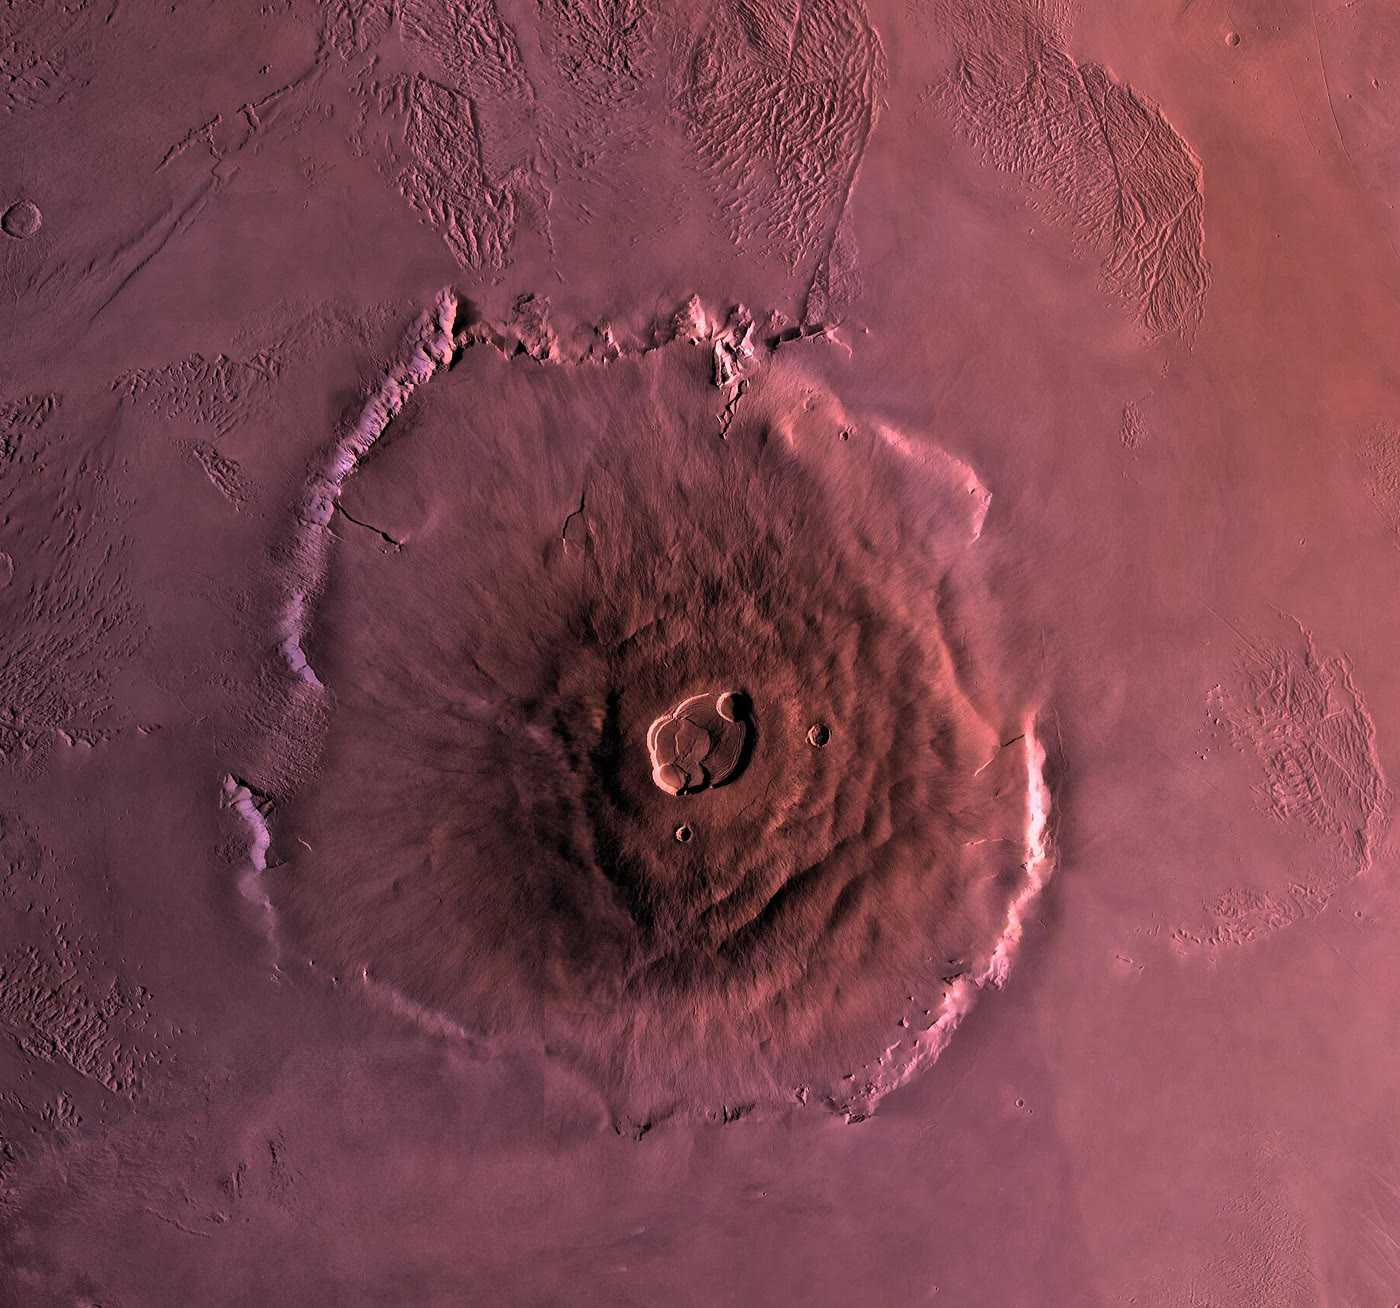
\includegraphics[width=0.48\linewidth]{images/book5/b3-olympus-mons.jpg}
\par\smallskip{\small Olympus Mons sur Mars, une mosaïque d'images des
orbiteurs Viking~: les calderas sommitales au centre, les flancs de coulées de lave et
l'escarpement en falaise qui cerne la base, large d'environ \qty{600}{km}.
NASA/JPL/USGS, domaine public.}\label{fig:b3:planetary-interiors-surfaces:olympus}
\end{omfigure}
% ledger: photo:b3-olympus-mons, nasa:olympus-mons

Vénus, la jumelle de la Terre par la taille, possède de loin le moins de cratères d'impact de
toute planète rocheuse à l'exception de la Terre. Ses formations de surface peuvent avoir en
moyenne un âge aussi jeune que 150 millions d'années, avec des zones plus anciennes entre elles~:
le volcanisme et la déformation ont renouvelé l'essentiel de sa surface, peut-être par morceaux
sur une longue durée, peut-être plus vite. Vénus compte des milliers de volcans et aucun signe
de plaques en mouvement.
% ledger: nasa:venus-surface, planet:Venus.diameter, planet:Earth.diameter

Io, la plus intérieure des grandes lunes de Jupiter, perd plus de
\qty{2.5}{W.m^{-2}} à travers sa surface, soit environ 27 fois la moyenne
terrestre de \qty{0.092}{W.m^{-2}}. Sa chaleur ne vient pas de la
radioactivité~: elle est produite par les marées.
% ledger: veeder:io-heat, dd10:split

\begin{definition}[Chauffage de marée]\label{def:b3:planetary-interiors-surfaces:tidal-heating}
Le \emph{chauffage de marée}\index{chauffage de marée} est la chaleur produite à l'intérieur
d'un corps par le frottement de la déformation que lui impose une marée variable.
Une lune en rotation synchrone sur une orbite excentrique voit la marée de sa
planète varier d'intensité et osciller d'avant en arrière au cours de chaque orbite.
\end{definition}

\begin{proposition}[Puissance de marée d'une lune synchrone]\label{prop:b3:planetary-interiors-surfaces:tidal-power}
Une lune de rayon $R$ en rotation synchrone, sur une orbite de moyen mouvement
$n$ et de faible excentricité $e$, dissipe la puissance
\[
  \dot E = \frac{21}{2}\,\frac{k_2}{Q}\,\frac{(nR)^5}{G}\,e^2 ,
\]
où $Q$ est le facteur de qualité de marée de la lune, de sorte que $k_2/Q$ mesure
la part de la déformation de marée perdue sous forme de chaleur.
\end{proposition}

La proposition est admise. Les marées qui dissipent de l'énergie arrondissent aussi
une orbite~; celle d'Io reste elliptique, d'excentricité 0.004, car les
attractions précisément synchronisées d'Europe et de Ganymède la perturbent, leurs
périodes orbitales de 1.77, 3.55 et \num{7.15}~jours restant presque exactement dans le
rapport 1:2:4 (l'\cref{exo:b3:planetary-interiors-surfaces:8}). Sa surface se soulève
et s'abaisse de \qty{100}{m} au plus à chaque orbite. Les volcans
recouvrent Io de lave plus vite que des cratères ne peuvent s'y former~; l'un des modèles de
dissipation de sa chaleur est le \omterm{def:b3:planetary-interiors-surfaces:heat-pipe}{volcanisme en caloduc}, qui maintiendrait une
lithosphère épaisse et froide sous sa surface brûlante.
% ledger: nasa:galilean-orbits, beuthe:tidal-power, nasa:io-orbit, nasa:io-facts

\begin{definition}[Océan souterrain]\label{def:b3:planetary-interiors-surfaces:ocean-world}
Un \emph{océan souterrain}\index{océan souterrain} est une couche globale d'eau
liquide sous la carapace de glace d'une lune ou d'une planète naine, maintenue à l'état
liquide par la chaleur de marée et la chaleur radiogénique.
\end{definition}

\begin{definition}[Cryovolcanisme]\label{def:b3:planetary-interiors-surfaces:cryovolcanism}
Le \emph{cryovolcanisme}\index{cryovolcanisme} est l'éruption d'eau, de saumures
ou d'autres liquides et vapeurs volatils, à la place de roche fondue, sur la
surface glacée d'une lune ou d'une planète naine.
\end{definition}

La carapace de glace d'Europe, mesurée par le radiomètre micro-ondes de la sonde Juno
dans la région qu'elle a survolée, mesure en moyenne environ \qty{29}{km} d'épaisseur~;
sous elle s'étend un océan salé contenant deux fois plus d'eau que l'ensemble des
océans terrestres. Sur Encelade, lune de Saturne qui ne mesure qu'environ \qty{500}{km}
de diamètre, la sonde Cassini a observé en 2005 des jets de grains de glace et de gaz
s'échappant de fractures chaudes près du pôle Sud à environ
\qty{400}{m.s^{-1}}. Sa gravité et les oscillations de sa rotation ont montré
que les jets puisent dans un océan global, sous une carapace de glace de 20 à
\qty{25}{km} d'épaisseur en moyenne et peut-être de seulement 1 à \qty{5}{km} au
pôle Sud.
% ledger: jpl:europa-shell, nasa:europa-ocean, nasa:enceladus

\section{Noyaux grands et petits}\label{sec:b3:planetary-interiors-surfaces:cores}

Les quatre noyaux mesurés forment une famille singulière. Rapporté à son rayon, le
noyau terrestre atteint 0.55 de la distance jusqu'à la surface, celui de Mars 0.54~;
celui de la Lune 0.19~; celui de Mercure 0.82. La différenciation, dans le volume de
deuxième année, sépare le métal du silicate à l'intérieur de chaque corps, mais ne peut rendre les
proportions de métal si différentes. Les impacts géants, eux, le peuvent. La Lune serait
née des débris d'une collision entre un corps de la taille de Mars et la jeune Terre, il y a
environ 4.5~Ga~; le métal de l'impacteur a rejoint le noyau terrestre tandis que la Lune a
surtout recueilli des roches du manteau, d'où son petit noyau. Des impacts semblables ont pu
arracher une grande part du manteau silicaté de Mercure et lui laisser cette planète riche
en fer dont le noyau occupe l'essentiel du volume.
Les noyaux, comme les cratères, gardent la trace d'une histoire de collisions.
% ledger: data:prem, jpl:insight-interior, nasa:moon-core, agu:mercury-core, french:giant-impacts

\section{Exercices}

\begin{exercise}[$\star$]\label{exo:b3:planetary-interiors-surfaces:1}
Mercure a une masse volumique moyenne de \qty{5429}{kg.m^{-3}}, un facteur de moment
d'inertie de 0.35 et un rayon de \qty{2440}{km}. Avec un modèle à deux couches et un
manteau de \qty{3300}{kg.m^{-3}}, calculer le rayon relatif du noyau, son rayon en
kilomètres et sa masse volumique.
\end{exercise}

\begin{exercise}[$\star$]\label{exo:b3:planetary-interiors-surfaces:2}
Un projectile rocheux de \qty{50}{m} de diamètre, de masse volumique \qty{3500}{kg.m^{-3}},
frappe la Terre à la verticale à \qty{20}{km.s^{-1}}. Calculer sa masse et
son énergie cinétique, en joules et en mégatonnes d'explosif
($\qty{1}{Mt} = \qty{4.2e15}{J}$). Quel diamètre de cratère donne la règle des
vingt diamètres de projectile~?
\end{exercise}

\begin{exercise}[$\star$]\label{exo:b3:planetary-interiors-surfaces:3}
Sur une plaine martienne de \qty{100000}{km^2}, on compte 120 cratères de \qty{1}{km} et
plus. Calculer $N_1$, son erreur relative, et l'âge modèle de la plaine
avec son erreur.
\end{exercise}

\begin{exercise}[$\star$]\label{exo:b3:planetary-interiors-surfaces:4}
Io, de rayon \qty{1821.5}{km}, perd \qty{2.5}{W.m^{-2}}. Calculer sa perte
de chaleur totale et la comparer à celle de la Terre, \qty{47}{TW}, en totalité et
par mètre carré (\qty{0.092}{W.m^{-2}}).
\end{exercise}

\begin{exercise}[$\star\star$]\label{exo:b3:planetary-interiors-surfaces:5}
Mars a une masse de \qty{6.417e23}{kg} et un rayon de \qty{3389.5}{km}.
(a)~Calculer sa masse volumique moyenne, sa gravité de surface et $\rho gR$.
(b)~En la considérant comme une sphère uniforme incompressible de rigidité
\qty{67}{GPa}, calculer son \omterm{def:b3:planetary-interiors-surfaces:love-number}{nombre de Love} $k_2$. (c)~La valeur mesurée est
$0.153 \pm 0.017$. Que dit la comparaison~?
\end{exercise}

\begin{exercise}[$\star\star$]\label{exo:b3:planetary-interiors-surfaces:6}
Sur la Terre ($g = \qty{9.8}{m.s^{-2}}$), la transition simple-complexe
se produit vers \qty{4}{km} dans la roche cristalline et \qty{2}{km} dans
les sédiments. (a)~En supposant que le diamètre de transition varie comme $1/g$,
prévoir sa valeur sur la Lune ($g = \qty{1.62}{m.s^{-2}}$) et sur Mars et
sur Mercure ($g = \qty{3.7}{m.s^{-2}}$)~; comparer avec les \qty{20}{km}
observés sur la Lune. (b)~Si l'effondrement commence lorsque $\rho gD/3$ dépasse la
résistance $Y$ de la roche, quelle résistance donne la transition cristalline de la Terre,
pour $\rho = \qty{2600}{kg.m^{-3}}$~?
\end{exercise}

\begin{exercise}[$\star\star$]\label{exo:b3:planetary-interiors-surfaces:7}
Une surface porte $\num{2.0e-3}$ cratères de \qty{1}{km} et plus par
kilomètre carré. Déterminer son âge modèle avec la fonction de chronologie de Mars,
en résolvant numériquement l'équation. Quel âge aurait donné la fonction lunaire
et pourquoi les deux fonctions ne peuvent-elles pas être échangées~?
\end{exercise}

\begin{exercise}[$\star\star$]\label{exo:b3:planetary-interiors-surfaces:8}
Les périodes orbitales d'Io, d'Europe et de Ganymède sont de 1.769138, 3.551181 et
\num{7.154553}~jours. (a)~Calculer les rapports des périodes successives.
(b)~Calculer $1/P_I - 3/P_E + 2/P_G$ et commenter. (c)~Pourquoi les résonances peuvent-elles
maintenir une excentricité que les marées feraient sinon disparaître~?
\end{exercise}

\begin{exercise}[$\star\star$]\label{exo:b3:planetary-interiors-surfaces:9}
Io orbite autour de Jupiter en \num{1.769138}~jours avec une excentricité de 0.004.
Calculer la puissance que fournit la proposition sur la puissance de marée, par unité de $k_2/Q$,
et la valeur de $k_2/Q$ qui fournirait la perte de chaleur
d'Io calculée dans l'\cref{exo:b3:planetary-interiors-surfaces:4}.
\end{exercise}

\begin{exercise}[$\star\star\star$]\label{exo:b3:planetary-interiors-surfaces:10}
Pour la Lune, $\bar\rho = \qty{3340}{kg.m^{-3}}$ et $C = 0.394$.
(a)~Montrer que dans le modèle à deux couches $\mathrm dx^2/\mathrm dC =
\tfrac52\bar\rho/(\bar\rho - \rho_m)$ à $\rho_m$ fixé. (b)~Avec la
masse volumique du manteau qui donne un noyau de $x = 0.19$, \qty{3288}{kg.m^{-3}},
quelles sont $x$ et $\rho_c$ pour $C = 0.395$, et pour $C = 0.393$~?
(c)~Que dit cela de la pesée d'un petit noyau à l'aide du moment
d'inertie~?
\end{exercise}

\begin{exercise}[$\star\star\star$]\label{exo:b3:planetary-interiors-surfaces:11}
(a)~Pour 100 cratères, calculer l'erreur de comptage de l'âge modèle
d'une surface martienne âgée de \qty{1.0}{Ga} et d'une autre âgée de \qty{3.8}{Ga}.
(b)~Montrer que sur la partie linéaire de la fonction de chronologie $\sigma_T/T =
1/\sqrt n$. (c)~Pourquoi les âges des surfaces anciennes restent-ils alors incertains~?
\end{exercise}

\begin{exercise}[$\star\star\star$]\label{exo:b3:planetary-interiors-surfaces:12}
Europe, de rayon \qty{1560.8}{km}, orbite en \num{3.551181}~jours avec
une excentricité de 0.009. (a)~Si Europe dissipait les marées avec le même $k_2/Q$
qu'Io, quelle fraction de la puissance de marée d'Io produirait-elle, et quel flux de chaleur~?
(b)~Pourquoi cette hypothèse est-elle douteuse pour une lune glacée abritant un \omterm{def:b3:planetary-interiors-surfaces:ocean-world}{océan souterrain}~?
\end{exercise}

\section{Problème~: deux plaines sur Mars}

\begin{problem}[{Problème du week-end --- le noyau de Mars et les âges de deux
plaines de lave inventées}]
\label{pb:b3:planetary-interiors-surfaces:1}
Mars a une masse de \qty{6.4169e23}{kg}, un rayon de \qty{3389.5}{km} et un
facteur de moment d'inertie de 0.366. Deux plaines inventées, A et B, se trouvent sur ses
provinces volcaniques~; leurs cratères ont été comptés sur des images en classes
de largeur $\sqrt2$.

\medskip\noindent\textbf{Partie I --- Le noyau.}
\begin{enumerate}
\item Calculer la masse volumique moyenne de Mars.
\item Avec un modèle à deux couches et un manteau de \qty{3500}{kg.m^{-3}}, calculer
  le rayon relatif du noyau, son rayon en kilomètres et sa
  masse volumique.
\item InSight a mesuré un rayon de noyau de \qty{1830}{km}. Quelles
  masses volumiques du manteau et du noyau le modèle à deux couches exige-t-il alors~?
\item Comparer cette masse volumique du noyau à celle du noyau externe de la Terre
  juste sous son sommet, \qty{9900}{kg.m^{-3}} dans le modèle de Terre de référence,
  et dire pourquoi une valeur plus faible est attendue pour Mars et ce qu'elle
  suggère d'autre.
\item Le \omterm{def:b3:planetary-interiors-surfaces:love-number}{nombre de Love} de Mars, pour une sphère uniforme de rigidité
  \qty{67}{GPa} vaut 0.109~; celui mesuré vaut 0.153. Quelle observation est
  arrivée en premier, et que disait-elle déjà du noyau~?
\item La croûte de Mars a une épaisseur de 20 à \qty{37}{km}. Quelle fraction du
  volume de la planète occupe-t-elle~? Était-il juste de la négliger~?
\end{enumerate}

\medskip\noindent\textbf{Partie II --- Les comptages sur la plaine A.} La plaine A
couvre \qty{80000}{km^2}. Ses cratères, par classe de diamètre (km)~:
\begin{center}
\small
\begin{tabular}{lccccccccc}
\hline
classe & 1--1.41 & 1.41--2 & 2--2.83 & 2.83--4 & 4--5.66 & 5.66--8 & 8--11.3 & 11.3--16 & 16--22.6 \\
\hline
plaine A & 38 & 6 & 5 & 3 & 0 & 0 & 0 & 1 & 1 \\
plaine B & 48 & 8 & 31 & 12 & 7 & 2 & 0 & 2 & 2 \\
\hline
\end{tabular}
\end{center}
\begin{enumerate}[resume]
\item Calculer les comptages cumulés de la plaine A, à partir de \qty{1}{km}.
\item Calculer $N(\qty{1}{km})$ par kilomètre carré ainsi que son
  écart-type.
\item La fonction de production donne $F(\qty{2}{km}) = 0.147$ et
  $F(\qty{1.41}{km}) = 0.355$. Les comptages à 1.41 et \qty{2}{km} sont-ils
  compatibles avec la forme de la fonction de production~?
\item La plaine A est-elle proche de la densité d'équilibre
  \qty{0.072}{km^{-2}} à \qty{1}{km}~?
\item Pourquoi les classes sont-elles choisies de largeur $\sqrt2$~?
\item Pourquoi les amas et les chaînes de petits cratères sont-ils exclus d'un comptage~?
\end{enumerate}

\medskip\noindent\textbf{Partie III --- Âges modèles.} Utiliser la
fonction de chronologie de Mars.
\begin{enumerate}[resume]
\item Calculer l'âge modèle de la plaine A. Vérifier que le terme exponentiel
  peut être négligé.
\item Calculer son erreur de comptage.
\item Quel âge aurait donné la chronologie lunaire~?
\item La plaine B couvre \qty{120000}{km^2}. En utilisant ses cratères de
  \qty{2}{km} et plus, calculer $N(\qty{2}{km})$, puis $N_1$, puis son âge modèle,
  en résolvant numériquement l'équation.
\item Calculer l'erreur de comptage de cet âge.
\item Comparer les erreurs relatives des deux âges et expliquer la
  différence.
\end{enumerate}

\medskip\noindent\textbf{Partie IV --- Les cratères enfouis de la plaine B.}
\begin{enumerate}[resume]
\item Combien de cratères entre 1 et \qty{2}{km} la plaine B devrait-elle compter si
  l'ensemble de sa surface avait l'âge de la question~16~? Combien en compte-t-elle réellement~?
\item Supposer que la lave a enfoui chaque cratère plus petit que \qty{2}{km} à un
  instant $T_r$ et a épargné les plus grands. Calculer $T_r$ à partir des
  cratères de \num{1}--\qty{2}{km}.
\item Calculer l'erreur de comptage de $T_r$.
\item Prendre un \omterm{def:b3:planetary-interiors-surfaces:crater-morphology}{cratère simple} frais sur Mars comme étant cinq fois moins profond que large
  (hypothèse de ce problème). Quelle épaisseur la lave doit-elle avoir pour enfouir un
  cratère de \qty{2}{km}, et pourquoi les plus grands apparaissent-ils encore~?
\item La lave de la plaine B et celle de la plaine A pourraient-elles appartenir
  à un même épisode de volcanisme~?
\item Donner l'âge modèle de la plaine A, en milliards d'années, à deux
  chiffres significatifs.
\end{enumerate}
\end{problem}
% ledger: nasa:mars, jpl:insight-interior, yoder:mars-k2, data:prem, craterstats:mars-pf, craterstats:mars-cf, craterstats:moon-cf, craterstats:equilibrium
